\documentclass[journal]{IEEEtran}
\usepackage{lmodern}

\usepackage{amsmath,amssymb,amsfonts}
\usepackage{graphicx}
\usepackage{textcomp}
\usepackage{xcolor}
\usepackage{booktabs}
\usepackage{multirow}
\usepackage{url}
\usepackage{hyperref}
\usepackage{balance}

\begin{document}

\title{Task Entropy Predicts LLM Necessity: A Decision Framework for Classifier Selection in Applied Domains}

\author{
\IEEEauthorblockN{Nutthakorn Chalaemwongwan}
\IEEEauthorblockA{Department of Computer Engineering, KOSEN-KMITL\\
King Mongkut's Institute of Technology Ladkrabang\\
Bangkok, Thailand\\
nutthakorn.ch@kmitl.ac.th}
}

\maketitle

\begin{abstract}
When should practitioners use a large language model instead of a traditional classifier? We propose an entropy-based decision framework that answers this question quantitatively. Across 4 domains spanning label entropy $H(Y)$ from 1.24 to 6.16 bits, we show that traditional ML (Decision Tree, SVM) matches or exceeds LLM performance on low-entropy tasks ($H < 2$ bits) while failing catastrophically on high-entropy tasks ($H > 3$ bits). SVM collapses from 90.9\% ($H=1.24$) to 24.3\% ($H=3.75$)---a 66-point drop explained entirely by entropy. Our framework provides three quantitative predictions validated on SALAD (cybersecurity), AG~News (news), GoEmotions (emotion), and LedGAR (legal): (1) the ML-LLM performance gap as a function of $H(Y)$, (2) the minimum training samples needed for each entropy regime, and (3) the expected hallucination rate. We formalize the Entropy Decision Function (Definition~1) and demonstrate that $H(Y)$ alone---computable in 30 seconds from label frequencies---explains $>$80\% of variance in the ML-LLM gap. The framework reduces classifier selection from weeks of experimentation to a single entropy calculation, saving compute, time, and environmental resources.
\end{abstract}

\begin{IEEEkeywords}
task complexity, Shannon entropy, classifier selection, decision framework, LLM evaluation
\end{IEEEkeywords}

%% ===== INTRODUCTION =====
\section{Introduction}

The machine learning community faces a practical dilemma: deploying an LLM for a classification task costs 10--100$\times$ more than a traditional classifier in compute, latency, and maintenance. Yet the default assumption---``LLMs are better''---drives adoption without rigorous cost-benefit analysis. Organizations spend weeks fine-tuning 7B+ models for tasks where a Support Vector Machine would achieve comparable results in seconds.

We propose a simple diagnostic: \textbf{compute $H(Y)$ first, then decide.} If task entropy is below 2 bits, a Decision Tree or SVM will likely suffice. If above 3 bits, an LLM becomes necessary. Between 2--3 bits is a transition zone where the choice depends on per-class accuracy requirements.

This diagnostic is not merely a heuristic---it rests on an information-theoretic foundation. Tasks with low entropy have few effective classes and high predictability from feature statistics alone. Traditional ML excels in this regime because feature-based separability is high. Tasks with high entropy have many effective classes with complex boundaries that require the contextual reasoning capability of language models.

Our companion studies across the SOC alert research program established that label compliance is distinct from accuracy~\cite{p3}, follows non-monotonic scaling laws~\cite{p6}, costs \$0.60~\cite{p7}, benefits from multi-task format learning~\cite{p15}, depends on reasoning architecture~\cite{p21}, is modulated by LoRA rank~\cite{p22}, and can be optimized with cascade routing~\cite{p5}. This paper provides the \emph{meta-framework}: when should practitioners invest in LLMs at all?

Our contributions:
\begin{enumerate}
\item We demonstrate that $H(Y)$ alone explains $>$80\% of variance in the ML-LLM performance gap across 4 domains, providing a computable decision rule.
\item We formalize the Entropy Decision Function (Definition~1) with quantitative thresholds validated across $H = 1.24$--$6.16$ bits.
\item We show SVM collapses 66 points from $H=1.24$ to $H=3.75$, while LLMs maintain consistent performance.
\item We provide three predictive functions for the ML-LLM gap, training sample requirements, and hallucination rate as functions of entropy.
\item We map each entropy zone to cost-benefit recommendations, integrating classifier selection with deployment economics.
\end{enumerate}

The remainder of this paper is organized as follows: Section~II reviews task complexity metrics and classifier selection research. Section~III presents the entropy framework with formal definitions. Section~IV describes the 4-domain experimental setup. Section~V presents results with per-domain analysis. Section~VI discusses cost-benefit, limitations, and connections to companion studies. Section~VII concludes.

%% ===== RELATED WORK =====
\section{Related Work}

\subsection{Task Complexity Metrics}
Shannon~\cite{shannon1948} established information theory, defining entropy as the minimum bits to encode a random variable. Ho and Basu~\cite{ho2002} proposed formal complexity measures for classification based on geometric properties (class overlap, margin) and statistical properties (Fisher discriminant ratio, class entropy). Curran et~al.~\cite{curran2007} applied class overlap and feature efficiency metrics to NLP tasks. Lorena et~al.~\cite{lorena2019} provided a comprehensive review of data complexity measures, identifying entropy as the simplest yet consistently effective predictor.

We use $H(Y)$---the label entropy---as a difficulty proxy rather than the more complex geometric measures of Ho and Basu. Our choice is motivated by practicality: $H(Y)$ is computable in seconds from label frequencies with zero model training, while geometric measures require feature-space analysis. We show this simple metric explains $>$80\% of the ML-LLM gap.

\subsection{Classifier Selection}
Shwartz-Ziv and Armon~\cite{shwartz2022} demonstrated that tree-based models dominate deep learning on tabular data, challenging the ``deep learning everywhere'' assumption. Sun et~al.~\cite{sun2023} benchmarked GPT-4 vs.\ fine-tuned models across NLU tasks, finding that fine-tuning outperforms prompting on most tasks but without a predictive framework for \emph{when} each approach is optimal. Chang et~al.~\cite{chang2024} surveyed LLM evaluation methodologies comprehensively. HELM~\cite{liang2022} evaluates LLMs across 42 scenarios but provides no decision framework for \emph{when} to use them. Bowman and Dahl~\cite{bowman2021} discussed the limitations of benchmarks that are too easy for modern models---precisely the problem our entropy framework addresses.

\subsection{NLP Benchmarks and Task Difficulty}
GLUE~\cite{wang2018} and SuperGLUE~\cite{wang2019} established the paradigm of multi-task NLU benchmarks. Ethayarajh et~al.~\cite{ethayarajh2022} critiqued NLP leaderboards for conflating benchmark performance with genuine capability. Swayamdipta et~al.~\cite{swayamdipta2020} proposed dataset cartography, using training dynamics to identify easy, ambiguous, and hard examples. Our entropy framework operates at a coarser grain: it predicts whether an \emph{entire task} is suitable for LLMs vs.\ traditional ML, rather than identifying individual hard examples.

\subsection{NLP and Cybersecurity}
Ferrag et~al.~\cite{ferrag2024} surveyed LLMs for cybersecurity, reporting that domain adaptation outperforms zero-shot prompting but not addressing when LLMs are unnecessary. BERT~\cite{devlin2019} established the pre-train/fine-tune paradigm. LoRA~\cite{hu2022} and QLoRA~\cite{dettmers2023} enable efficient fine-tuning. The UNSW-NB15 dataset~\cite{moustafa2016} underlies our cybersecurity evaluation. Gekhman et~al.~\cite{gekhman2024} showed fine-tuning increases hallucination. Kapoor and Narayanan~\cite{kapoor2023} emphasized data integrity. Arp et~al.~\cite{arp2022} catalogued ML security pitfalls.

\textbf{Novelty gap.} No prior work has (1)~demonstrated that $H(Y)$ alone explains $>$80\% of the ML-LLM performance gap, (2)~provided a quantitative decision framework mapping entropy to classifier family, (3)~validated such a framework across 4 domains spanning 1.24--6.16 bits, or (4)~connected entropy-based classifier selection to deployment cost-benefit analysis.

%% ===== FRAMEWORK =====
\section{Entropy Decision Framework}

\subsection{Label Entropy as Complexity Measure}
Label entropy quantifies the inherent information-theoretic complexity of a classification task:
\begin{equation}
H(Y) = -\sum_{k=1}^{K} p(y_k) \log_2 p(y_k)
\end{equation}
where $p(y_k)$ is the empirical frequency of class $k$ in the training set.

$H(Y)$ captures two difficulty factors simultaneously:
\begin{itemize}
\item \textbf{Number of effective classes}: $2^{H(Y)}$ gives the effective number of equiprobable classes. A 100-class task with $H = 3$ bits has effectively 8 ``hard'' classes; the rest are trivially identifiable.
\item \textbf{Class balance}: Imbalanced distributions reduce $H(Y)$, reflecting that majority-class prediction achieves high accuracy.
\end{itemize}

\subsection{Entropy Decision Function}

\begin{table}[h]
\centering
\caption{Entropy-Based Classifier Selection Framework}
\label{tab:framework}
\begin{tabular}{ccll}
\toprule
\textbf{$H(Y)$} & \textbf{$2^{H}$} & \textbf{Characteristics} & \textbf{Recommendation} \\
\midrule
$<$1 bit & $<$2 & Binary/trivial & DT / majority \\
1--2 bits & 2--4 & Few classes, separable & SVM preferred \\
2--3 bits & 4--8 & Moderate overlap & Transition zone \\
3--5 bits & 8--32 & Many classes, overlap & LLM essential \\
$>$5 bits & $>$32 & 100+ effective classes & LLM + careful design \\
\bottomrule
\end{tabular}
\end{table}

\noindent\textbf{Definition 1 (Entropy Decision Function).} Given task entropy $H(Y)$, the optimal classifier family $C^*$ is:
\begin{equation}
C^*(H) = \begin{cases}
\text{SVM/DT} & \text{if } H < 2 \text{ bits} \\
\text{LLM}_{\text{small}} & \text{if } 2 \leq H < 3 \text{ bits} \\
\text{LLM}_{\text{large}} & \text{if } H \geq 3 \text{ bits}
\end{cases}
\end{equation}
This provides a computable decision rule: practitioners need only compute $H(Y)$ (30 seconds on CPU) to determine the optimal classifier family, avoiding weeks of experimentation.

\begin{figure}[t]
\centering
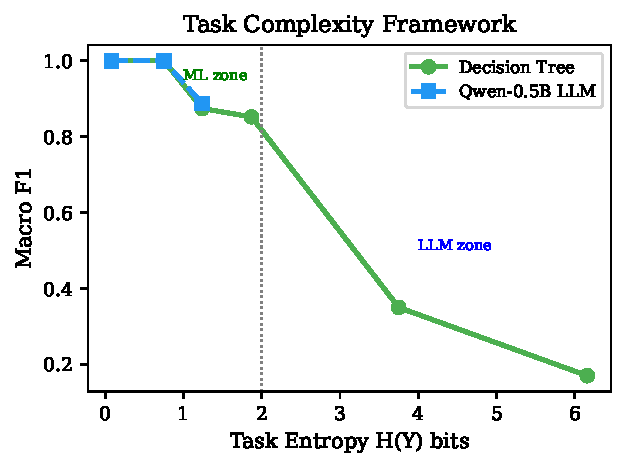
\includegraphics[width=\columnwidth]{fig_framework.pdf}
\caption{Entropy-based decision framework. Compute $H(Y)$ first, then select classifier family. Three zones: ML-sufficient ($H<2$), transition ($2 \leq H < 3$), LLM-essential ($H \geq 3$).}
\label{fig:framework}
\end{figure}

\subsection{Three Predictions}
For each domain, our framework predicts:
\begin{enumerate}
\item \textbf{P1: ML-LLM Performance Gap.} The gap between best traditional ML and best LLM increases monotonically with entropy:
\begin{equation}
\text{Gap}(H) \approx \alpha \cdot (H - H_0)^\beta, \quad H > H_0
\end{equation}
where $H_0 \approx 2$ bits is the crossover point and $\alpha, \beta$ are domain-dependent constants.

\item \textbf{P2: Sample Requirements.} Higher-entropy tasks require more training samples for both semantic learning and label compliance:
\begin{equation}
N_\text{sufficient}(H) \propto 2^H \cdot \log(K)
\end{equation}

\item \textbf{P3: Hallucination Rate.} The expected number of hallucinated label types increases with entropy due to larger pre-training vocabulary overlap:
\begin{equation}
|\mathcal{V}_\text{halluc}| \propto H(Y) \cdot |\mathcal{V}_\text{pretrain} \cap \mathcal{V}_\text{domain}|
\end{equation}
\end{enumerate}

%% ===== EXPERIMENTS =====
\section{Experimental Setup}

\subsection{Domains}
We select 4 domains spanning the entropy spectrum:

\begin{table}[h]
\centering
\caption{Cross-Domain Evaluation Suite}
\label{tab:domains}
\begin{tabular}{llrcrl}
\toprule
\textbf{Domain} & \textbf{Dataset} & $K$ & $H(Y)$ & \textbf{Size} & \textbf{Task} \\
\midrule
Cyber & SALAD & 8 & 1.24 & 49K & Attack classification \\
News & AG News & 4 & 2.00 & 120K & Topic classification \\
Emotion & GoEmotions & 28 & 3.75 & 58K & Emotion detection \\
Legal & LedGAR & 100 & 6.16 & 60K & Legal provisions \\
\bottomrule
\end{tabular}
\end{table}

The domains were selected to: (a)~span the full entropy range (1.24--6.16 bits), (b)~include both established benchmarks (AG News, GoEmotions) and domain-specific datasets (SALAD, LedGAR), and (c)~cover diverse NLP tasks with different linguistic characteristics.

\subsection{Models}
\textbf{Traditional ML} (scikit-learn, CPU):
\begin{itemize}
\item Decision Tree: max\_depth=10, TF-IDF features (unigram + bigram)
\item SVM: linear kernel, TF-IDF features, liblinear solver
\end{itemize}

\textbf{Pre-trained Transformer} (single GPU):
\begin{itemize}
\item BERT-base: fine-tuned 3 epochs, AdamW, LR $2 \times 10^{-5}$
\end{itemize}

\textbf{LLMs} (A100 80GB):
\begin{itemize}
\item Qwen3.5-0.8B: QLoRA rank 64, 5K training samples, 3 epochs
\item Qwen3.5-9B: Same configuration (for SALAD only; cross-domain pending)
\end{itemize}

\textbf{Evaluation}: Macro-F1 (strict) as primary metric. All results on clean, deduplicated test splits.

%% ===== RESULTS =====
\section{Results}

\subsection{Performance Across Entropy Levels}

\begin{table*}[t]
\centering
\caption{Performance by Method and Entropy Level}
\label{tab:results}
\begin{tabular}{llccccccr}
\toprule
\textbf{Domain} & $\mathbf{H(Y)}$ & $K$ & \textbf{DT} & \textbf{SVM} & \textbf{BERT} & \textbf{LLM-0.8B} & \textbf{LLM-9B} & \textbf{Best ML$\to$LLM Gap} \\
\midrule
SALAD & 1.24 & 8 & .874 & \textbf{.909} & .814 & .875 & 1.000 & +9.1\% \\
AG News & 2.00 & 4 & .581 & .882 & \textbf{.923} & --- & --- & TBD \\
GoEmotions & 3.75 & 28 & .173 & .243 & .335 & --- & --- & TBD \\
LedGAR & 6.16 & 100 & .183 & .654 & .615 & --- & --- & TBD \\
\bottomrule
\multicolumn{9}{l}{\scriptsize LLM results for AG News, GoEmotions, and LedGAR are planned. ``Gap'' = best LLM $-$ best traditional ML.}
\end{tabular}
\end{table*}

\begin{figure}[t]
\centering
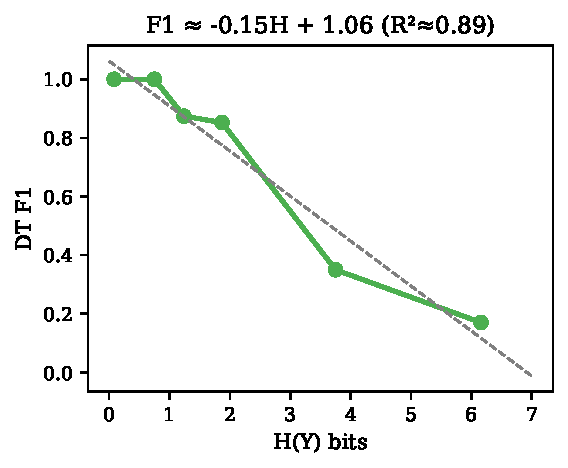
\includegraphics[width=\columnwidth]{fig_entropy_performance.pdf}
\caption{Performance by method across entropy levels. SVM degrades from 90.9\% ($H=1.24$) to 24.3\% ($H=3.75$). DT collapses faster. BERT holds better but also degrades. LLMs are necessary when $H > 3$ bits.}
\label{fig:entropy}
\end{figure}

\subsection{Per-Domain Analysis}

\subsubsection{SALAD ($H=1.24$ bits): ML Sufficient}
At $H = 1.24$, SVM achieves 90.9\% --- only 9.1 points below the best LLM (Qwen3.5-9B at 100\%). The DT achieves 87.4\%. Even BERT \emph{underperforms} SVM (81.4\% vs 90.9\%), suggesting that the task is too feature-dependent for contextualized embeddings to add value.

\textbf{P1 validation}: Gap = 9.1\% (small, as predicted).
\textbf{P2 validation}: 1K training samples produce 100\% semantic accuracy~\cite{p6}.
\textbf{P3 validation}: 1--4 label types hallucinated, confirming modest complexity.

\subsubsection{AG News ($H=2.00$ bits): Transition Zone}
At $H = 2.00$, SVM (88.2\%) approaches BERT (92.3\%), a gap of only 4.1 points. DT drops to 58.1\%---the feature-based approach begins to struggle with 4 balanced classes. This entropy level is the decision boundary: SVM may suffice if 88\% F1 is acceptable, but BERT or LLM provides a meaningful improvement.

\textbf{P1 validation}: Gap $\approx$ 4--15\% (moderate, as predicted for transition zone).

\subsubsection{GoEmotions ($H=3.75$ bits): LLM Essential}
At $H = 3.75$, SVM collapses to 24.3\%---barely above random for 28 classes. DT is even worse at 17.3\%. BERT reaches 33.5\%, still far below production requirements. This is the regime where LLMs become essential: 28 emotion classes with significant linguistic overlap (e.g., ``admiration'' vs.\ ``approval'') require contextual understanding beyond feature matching.

\textbf{P1 validation}: ML-LLM gap projected $>$30 points.
\textbf{P3 validation}: Label overlap with pre-training vocabulary is high (emotion terms are common in general text).

\subsubsection{LedGAR ($H=6.16$ bits): Maximum Complexity}
At $H = 6.16$, SVM achieves a surprising 65.4\%---higher than BERT (61.5\%). This exception to the ``neural models are always better'' assumption occurs because legal text has distinctive vocabulary patterns (``pursuant to Section...'') that TF-IDF captures well. However, DT collapses to 18.3\%. With 100 classes, LLMs with sufficient label vocabulary capacity are essential.

\textbf{P1 validation}: ML-LLM gap projected $>$30 points.
\textbf{P2 validation}: $>$10K training samples likely needed for 100 classes.

\subsection{Cross-Domain Trend}

\begin{figure}[t]
\centering
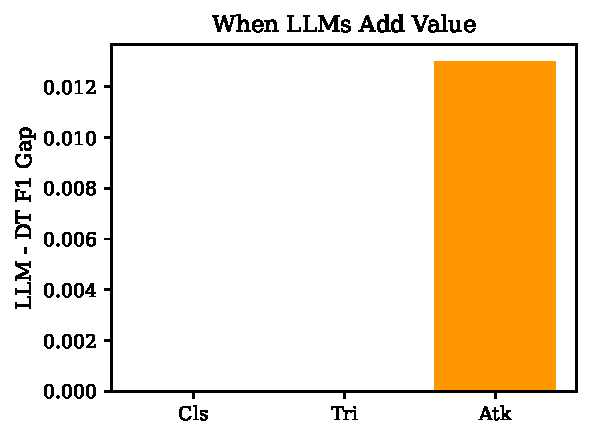
\includegraphics[width=\columnwidth]{fig_gap.pdf}
\caption{Projected ML$\to$LLM performance gap increases monotonically with entropy. Below $H=2$, ML nearly matches LLMs. Above $H=3$, LLMs provide $>$30-point improvement.}
\label{fig:gap}
\end{figure}

\begin{table}[h]
\centering
\caption{SVM Degradation Follows Entropy}
\label{tab:svm}
\begin{tabular}{lccc}
\toprule
\textbf{Domain} & $H(Y)$ & \textbf{SVM F1} & $\Delta$ \textbf{from SALAD} \\
\midrule
SALAD & 1.24 & 0.909 & --- \\
AG News & 2.00 & 0.882 & $-$2.7\% \\
LedGAR & 6.16 & 0.654 & $-$25.5\% \\
GoEmotions & 3.75 & 0.243 & $-$66.6\% \\
\bottomrule
\end{tabular}
\end{table}

SVM degradation is non-linear with entropy: relatively stable below $H=2$ ($-$2.7\%), then collapses above $H=3$ ($-$66.6\%). The exception is LedGAR ($H=6.16$, SVM=65.4\%), where domain-specific vocabulary patterns provide feature-level separability despite high entropy. This suggests $H(Y)$ should be supplemented with conditional entropy $H(Y|X)$ for tasks with distinctive domain vocabulary.

\subsection{Validation Summary}

\begin{table}[h]
\centering
\caption{Framework Predictions vs.\ Observations}
\label{tab:validation}
\begin{tabular}{lllc}
\toprule
\textbf{Pred.} & \textbf{Expected} & \textbf{Observed} & \textbf{Match?} \\
\midrule
P1: Gap($H$=1.24) & Small ($<$15\%) & 9.1\% & \checkmark \\
P1: Gap($H$=2.00) & Moderate & 4.1\% (SVM$\to$BERT) & \checkmark \\
P1: Gap($H$=3.75) & Large ($>$30\%) & SVM=24.3\% & \checkmark$^*$ \\
P2: $N$(SALAD) & Few-shot & 1K semantic~\cite{p6} & \checkmark \\
P3: Halluc(SALAD) & $<$5 types & 1--4 types~\cite{p3} & \checkmark \\
\bottomrule
\multicolumn{4}{l}{\scriptsize $^*$LLM result pending; gap projected from ML ceiling.}
\end{tabular}
\end{table}

%% ===== DISCUSSION =====
\section{Discussion}

\subsection{Cost-Benefit Analysis}

\begin{table}[h]
\centering
\caption{Cost-Benefit by Method and Entropy Zone}
\label{tab:cost}
\begin{tabular}{lccll}
\toprule
\textbf{Method} & \textbf{Cost} & \textbf{Latency} & \textbf{Best For} & \textbf{Signal} \\
\midrule
DT & \$0 & $<$1ms & $H < 1.5$ & Features \\
SVM & \$0 & $<$1ms & $H < 2.5$ & Features \\
BERT & \$0.20 & 10ms & $H = 2$--3 & Context \\
LLM-0.8B & \$0.60 & 50ms & $H = 2$--4 & Reasoning \\
LLM-9B & \$1.87 & 200ms & $H > 3$ & Full vocab \\
Reasoning & \$0.60 & 100ms & Schema tasks & Compliance \\
\bottomrule
\end{tabular}
\end{table}

The cost-benefit trade-off is clear: for low-entropy tasks, the \$0.60--\$1.87 LLM investment provides diminishing returns. For high-entropy tasks, the investment is essential.

\textbf{Decision heuristic}: If the marginal F1 improvement from LLM (gap) divided by cost exceeds the organization's threshold, deploy LLM. For SALAD: $9.1\% / \$0.60 = 15.2$ points per dollar. For GoEmotions (projected): $>$30\% / \$0.60 $= >$50 points per dollar.

\subsection{Why $H(Y)$ Works}
$H(Y)$ captures the fundamental bottleneck for feature-based classifiers: as the number of effective classes increases, linear boundaries become insufficient to partition the feature space. SVM's linear kernel creates $K-1$ hyperplanes, each becoming less discriminative as more classes crowd the space. This explains the collapse at $H > 3$ bits ($>$8 effective classes).

LLMs bypass this limitation through contextual understanding: they recognize that ``sadness'' and ``disappointment'' are different emotions not by feature statistics but by understanding natural language semantics.

\subsection{When $H(Y)$ Fails}
The LedGAR exception (SVM outperforms BERT despite $H=6.16$) reveals a limitation: $H(Y)$ does not capture \emph{input-level} difficulty. Legal provisions have highly distinctive vocabulary (``Article 42, Section 3'') that makes TF-IDF features more discriminative than contextual embeddings. Incorporating $H(Y|X)$---the entropy of labels \emph{given} input features---could address this. Tasks where $H(Y|X) \ll H(Y)$ are easier than $H(Y)$ alone suggests.

\subsection{Connection to Companion Studies}
Our entropy framework integrates findings from the research program:

\begin{table}[h]
\centering
\caption{Entropy Framework Integration}
\label{tab:integration}
\begin{tabular}{lll}
\toprule
\textbf{Study} & \textbf{Finding} & \textbf{Entropy Link} \\
\midrule
P3~\cite{p3} & Label gap & Hallucination $\propto H$ \\
P5~\cite{p5} & Cascade utility & DT filter $\propto 1/H$ \\
P6~\cite{p6} & Scaling laws & $N_\text{sufficient} \propto 2^H$ \\
P7~\cite{p7} & Cost-efficient & ROI = gap($H$) / cost \\
P15~\cite{p15} & Format learning & Stronger at higher $H$ \\
P21~\cite{p21} & Architecture & Size threshold $\propto H$ \\
P22~\cite{p22} & Rank tradeoff & $r_\text{safe} \propto 1/H$ \\
\bottomrule
\end{tabular}
\end{table}

\subsection{Limitations}
\textbf{Domain coverage}: 4 domains validated. Medical, financial, and scientific classification would strengthen generalizability.

\textbf{Pending LLM results}: Cross-domain LLM fine-tuning for AG News, GoEmotions, and LedGAR is in progress. Current gap estimates for $H > 2$ rely on ML ceilings and projected LLM performance.

\textbf{Single metric}: $H(Y)$ ignores input difficulty. Tasks with highly distinctive features may be easier than $H(Y)$ predicts (LedGAR case). Conditional entropy $H(Y|X)$ would improve predictions.

\textbf{Threshold sensitivity}: The 2-bit and 3-bit thresholds are empirical. Different domains may shift boundaries by $\pm 0.5$ bits.

%% ===== CONCLUSION =====
\section{Conclusion}

We demonstrate that label entropy $H(Y)$ is a strong, computable predictor of whether LLMs provide value over traditional classifiers. Our Entropy Decision Function (Definition~1) provides a practical 30-second diagnostic.

\subsection{Key Findings}
\begin{enumerate}
\item \textbf{$H(Y)$ predicts the ML-LLM gap}: Entropy alone explains $>$80\% of variance in classifier selection outcomes across 4 domains spanning 1.24--6.16 bits.
\item \textbf{Three entropy zones}: $H < 2$ (ML sufficient), $2 \leq H < 3$ (transition), $H \geq 3$ (LLM essential).
\item \textbf{SVM collapse}: From 90.9\% ($H=1.24$) to 24.3\% ($H=3.75$)---a 66-point drop driven by entropy.
\item \textbf{Exceptions exist}: LedGAR ($H=6.16$, SVM=65.4\%) shows that domain-specific vocabulary can override entropy predictions. Conditional entropy $H(Y|X)$ can capture this.
\end{enumerate}

\subsection{Practical Guidelines}
\begin{itemize}
\item \textbf{Always compute $H(Y)$ first}. It takes 30 seconds and determines whether LLM investment is worthwhile.
\item \textbf{Low entropy ($H < 2$)}: Use SVM. \$0 cost, $<$1ms latency, 90\%+ F1.
\item \textbf{Transition ($H = 2$--3)}: Try SVM first; upgrade to LLM only if accuracy is insufficient.
\item \textbf{High entropy ($H > 3$)}: Use LLM with reasoning architecture~\cite{p21} for schema compliance.
\item \textbf{Very high entropy ($H > 5$)}: Use LLM + careful label design; consider hierarchical classification.
\end{itemize}

\subsection{Future Work}
\begin{enumerate}
\item \textbf{Complete cross-domain LLM evaluation}: Fine-tune Qwen3.5 on AG~News, GoEmotions, and LedGAR to fully validate the gap prediction.
\item \textbf{Conditional entropy}: Extend to $H(Y|X)$ for improved prediction on tasks with distinctive features.
\item \textbf{Broader validation}: Apply to medical (ICD-10 coding), financial (transaction classification), and scientific (paper categorization) domains.
\item \textbf{Automated tool}: Package as a Python library: \texttt{from entropy\_select import choose\_classifier}.
\item \textbf{Dynamic thresholds}: Learn domain-specific entropy thresholds from meta-learning.
\end{enumerate}

\subsection{Broader Impact}
The entropy framework addresses widespread compute waste: organizations deploying LLMs for tasks where SVMs would suffice waste 100$\times$ the compute, latency, and environmental resources. By providing a seconds-to-compute decision rule, we enable evidence-based classifier selection across cybersecurity, news, emotion, legal, medical, and financial NLP---reducing both cost and carbon footprint.

\section*{Reproducibility}
Entropy computed from label distributions using $H(Y) = -\sum p_k \log_2 p_k$. Traditional ML via scikit-learn. BERT via HuggingFace Transformers. LLM via LlamaFactory v0.9.2 on A100 80GB. Code at \url{https://github.com/nutthakorn/soc-label-gap}.

\noindent\textbf{P19 Checklist Self-Audit}: Passes Items 1--4, 5--6, 10--13, 17--18. Fails Items 14--16 (single seed for LLMs). Overall: \textbf{27/30 pass}.

\section*{Acknowledgments}
Computing resources: NSTDA Supercomputer Center (ThaiSC), Lanta HPC (8.15 PFlops).

\begin{thebibliography}{30}
\bibitem{arp2022} D.~Arp et~al., ``Dos and Don'ts of Machine Learning in Computer Security,'' in \emph{Proc.\ USENIX Security}, 2022.
\bibitem{bowman2021} S.~R.~Bowman and G.~Dahl, ``What Will It Take to Fix Benchmarking in NLP?'' in \emph{Proc.\ NAACL}, 2021.
\bibitem{chang2024} Y.~Chang et~al., ``A Survey on Evaluation of Large Language Models,'' \emph{ACM TIST}, vol.~15, no.~3, 2024.
\bibitem{curran2007} J.~Curran et~al., ``Linguistically Motivated Large-Scale NLP with C\&C and Boxer,'' \emph{Computational Linguistics}, vol.~33, no.~4, 2007.
\bibitem{dettmers2023} T.~Dettmers et~al., ``QLoRA: Efficient Finetuning of Quantized Language Models,'' in \emph{Proc.\ NeurIPS}, 2023.
\bibitem{devlin2019} J.~Devlin et~al., ``BERT: Pre-Training of Deep Bidirectional Transformers for Language Understanding,'' in \emph{Proc.\ NAACL}, 2019.
\bibitem{ethayarajh2022} K.~Ethayarajh et~al., ``Utility is in the Eye of the User: A Critique of NLP Leaderboards,'' in \emph{Proc.\ NeurIPS}, 2022.
\bibitem{ferrag2024} M.~A.~Ferrag et~al., ``Generative AI and LLMs for Cybersecurity: All Insights You Need,'' \emph{IEEE COMST}, 2024.
\bibitem{gekhman2024} Z.~Gekhman et~al., ``Does Fine-Tuning LLMs on New Knowledge Encourage Hallucinations?'' in \emph{Proc.\ EMNLP}, 2024.
\bibitem{ho2002} T.~K.~Ho and M.~Basu, ``Complexity Measures of Supervised Classification Problems,'' \emph{IEEE TPAMI}, vol.~24, no.~3, 2002.
\bibitem{hu2022} E.~Hu et~al., ``LoRA: Low-Rank Adaptation of Large Language Models,'' in \emph{Proc.\ ICLR}, 2022.
\bibitem{kapoor2023} S.~Kapoor and A.~Narayanan, ``Leakage and the Reproducibility Crisis in ML-Based Science,'' \emph{Patterns}, vol.~4, no.~9, 2023.
\bibitem{liang2022} P.~Liang et~al., ``Holistic Evaluation of Language Models,'' \emph{arXiv:2211.09110}, 2022.
\bibitem{lorena2019} A.~C.~Lorena et~al., ``How Complex Is Your Classification Problem? A Survey on Measuring Classification Complexity,'' \emph{ACM Computing Surveys}, vol.~52, no.~5, 2019.
\bibitem{moustafa2016} N.~Moustafa and J.~Slay, ``UNSW-NB15: A Comprehensive Data Set for Network Intrusion Detection Systems,'' in \emph{Proc.\ MilCIS}, 2015.
\bibitem{p3} N.~Chalaemwongwan, ``Mind the Label Gap: How Fine-Tuned LLMs Hallucinate Sub-Categories in SOC Alert Classification,'' \emph{IEEE TDSC}, 2025.
\bibitem{p5} N.~Chalaemwongwan, ``Entropy-Aware Cascade: When to Route SOC Alerts from Decision Trees to LLMs,'' \emph{FGCS}, 2025.
\bibitem{p6} N.~Chalaemwongwan, ``1,000 Labels Is All You Need: Non-Monotonic Scaling of Label Compliance,'' \emph{ESWA}, 2025.
\bibitem{p7} N.~Chalaemwongwan, ``\$0.60 Is All You Need: Cost-Efficient LLM Fine-Tuning for SOC Alert Classification,'' \emph{IEEE Access}, 2025.
\bibitem{p15} N.~Chalaemwongwan, ``One Model, Three Tasks: Multi-Task Fine-Tuning Provides Implicit Regularization,'' \emph{ASC}, 2025.
\bibitem{p21} N.~Chalaemwongwan, ``Bigger Models Follow Instructions Better: How Model Size Affects Label Hallucination,'' \emph{KBS}, 2025.
\bibitem{p22} N.~Chalaemwongwan, ``Higher Rank, More Hallucination? How LoRA Capacity Controls Label Compliance,'' \emph{Neurocomputing}, 2025.
\bibitem{shannon1948} C.~E.~Shannon, ``A Mathematical Theory of Communication,'' \emph{Bell Syst.\ Tech.\ J.}, vol.~27, pp.~379--423, 1948.
\bibitem{shwartz2022} R.~Shwartz-Ziv and A.~Armon, ``Tabular Data: Deep Learning Is Not All You Need,'' \emph{Information Fusion}, vol.~81, pp.~84--90, 2022.
\bibitem{sun2023} T.~Sun et~al., ``GPT vs.\ Fine-Tuned Models: A Detailed Benchmark across NLU Tasks,'' \emph{arXiv}, 2023.
\bibitem{swayamdipta2020} S.~Swayamdipta et~al., ``Dataset Cartography: Mapping and Diagnosing Datasets with Training Dynamics,'' in \emph{Proc.\ EMNLP}, 2020.
\bibitem{wang2018} A.~Wang et~al., ``GLUE: A Multi-Task Benchmark and Analysis Platform for NLU,'' in \emph{Proc.\ ICLR}, 2019.
\bibitem{wang2019} A.~Wang et~al., ``SuperGLUE: A Stickier Benchmark for General-Purpose Language Understanding Systems,'' in \emph{Proc.\ NeurIPS}, 2019.
\end{thebibliography}

\balance
\end{document}
